\documentclass[12pt,twoside]{manual}






%%######################################################################
%% Styles
%%######################################################################

\tikzstyle{parentIsotope} = [rectangle, rounded corners, minimum width=3cm, minimum height=1cm,text centered, draw=black, fill=white]
\tikzstyle{unstableIsotope} = [rectangle, minimum width=3cm, minimum height=1cm,text centered, draw=black, fill=white]
\tikzstyle{stableIsotope} = [rectangle, rounded corners, minimum width=3cm, minimum height=1cm,text centered, draw=black, fill=white]
\tikzstyle{isotopeProduction} = [rectangle, minimum width=3cm, minimum height=1cm,text centered, draw=black, fill=white]

\tikzstyle{decision} = [diamond, draw, fill=blue!20, text width=4.5em, text badly centered, node distance=3cm, inner sep=0pt]
\tikzstyle{block} = [rectangle, draw, fill=blue!20, text width=5em, text centered, rounded corners, minimum height=4em]
\tikzstyle{line} = [draw, -latex']
\tikzstyle{cloud} = [draw, ellipse,fill=red!20, node distance=3cm, minimum height=2em]

\tikzstyle{startstop} = [rectangle, rounded corners, minimum width=3cm, minimum height=1cm,text centered, draw=black, fill=grey!30]
\tikzstyle{process} = [rectangle, minimum width=3cm, minimum height=1cm, text centered, draw=black, fill=grey!10]
\tikzstyle{decision} = [diamond, minimum width=3cm, minimum height=1cm, text centered, draw=black, fill=grey!10]
\tikzstyle{arrow} = [thick,->]



%%######################################################################
%% Listings
%%######################################################################

\usepackage{listings}
\lstloadlanguages{Fortran,Bash,Python,C++}
\lstloadlanguages{Matlab}

\lstdefinestyle{inputfile}
{
  breaklines=true,
  numbers=left,
  stepnumber=1,
  tabsize=4,
  numberstyle=\tiny\color{gray},
  keywordstyle=\color{blue},
  commentstyle=\color{dkgreen},
  stringstyle=\color{mauve}
}

\lstdefinestyle{spython}
{
	language=Python,
  breaklines=true,
  numbers=left,
  stepnumber=1,
  tabsize=4,
  numberstyle=\tiny\color{gray},
  keywordstyle=\color{blue},
  commentstyle=\color{dkgreen},
  stringstyle=\color{mauve}
}

\lstdefinestyle{pseudocode}
{
  breaklines=true,
  numbers=left,
  stepnumber=1,
  tabsize=4,
  keywordstyle=\color{blue}
}









\definecolor{col_336699}{RGB}{51,102,153}
\definecolor{col_333333}{RGB}{51,51,51}
\definecolor{col_111111}{RGB}{17,17,17}
\definecolor{col_555555}{RGB}{85,85,85}
\definecolor{col_666666}{RGB}{102,102,102}
\definecolor{col_777777}{RGB}{119,119,119}
\definecolor{col_000022}{RGB}{0,0,34}
\definecolor{col_000000}{RGB}{0,0,0}


 
%% DRAW LINE
\newcommand{\tikzdrawline}[7]{
\draw[#1] (#2,#4,#3) -- (#5,#7,#6);  
}
%% DRAW BALL
\newcommand{\tikzdrawatom}[5]{%
\filldraw[ball color=#1] (#2,#3,#4) circle[radius=#5];
}  

%% DRAW ARROW
\newcommand{\tikzdrawarrow}[9]{
\draw[#1, thick, ->] (#2,#4,#3) -- (#5,#7,#6) node[midway,#8]{#9};  
}

\newcommand{\tikzdrawlinethick}[7]{
\draw[#1, line width=0.5mm] (#2,#4,#3) -- (#5,#7,#6);  
} 

\newcommand{\tikzdrawlinedotted}[7]{
\draw[#1, dotted] (#2,#4,#3) -- (#5,#7,#6);  
}

%% DRAW COORD GRID
\newcommand{\tikzcoordgrid}[6]{%
\fill[col_336699!10,opacity=1.0] (0.0,0.0,0.0) -- (0.0,0.0,#1) -- (0.0,#3,#1) -- (0.0,#3,0.0) -- cycle;
\fill[col_336699!15,opacity=1.0] (0.0,0.0,0.0) -- (0.0,#3,0.0) -- (#2,#3,0.0) -- (#2,0.0,0.0) -- cycle;
\fill[col_336699!30,opacity=1.0] (0.0,0.0,0.0) -- (#2,0.0,0.0) -- (#2,0.0,#1) -- (0.0,0.0,#1) -- cycle;
\tikzdrawarrow{col_000000}{0.0}{0.0}{0.0}{0.0}{1.05*#1}{0.0}{above}{#4};
\tikzdrawarrow{col_000000}{0.0}{0.0}{0.0}{1.05*#1}{0.0}{0.0}{above}{#5};
\tikzdrawarrow{col_000000}{0.0}{0.0}{0.0}{0.0}{0.0}{1.05*#1}{left}{#6};
}  





\pagestyle{plain}
\begin{document}


%%######################################################################
%% Cover Page
%%######################################################################

\begin{titlepage}
  \begin{center}
    \centerline{
\includegraphics[width=0.7\textwidth]{img/coverart}}


    \textbf{Department of Metallurgy \& Materials}

    \vspace*{2.0cm}
    \Large{}
    \textbf{EAMPA Manual}
    \textbf{EAM Potential Anayser (and fitting)}
    \vspace{0.8cm}
    \normalsize{}

  \end{center}
\end{titlepage}

\pagenumbering{gobble}

\pagenumbering{roman} 

\tableofcontents

\pagenumbering{arabic}







%%######################################################################
%% Introduction
%%######################################################################

\chapter{Introduction}

\section{What does it do?}

This code takes a potential function or set of functions as an input.  Given a set of atom configurations this code will:

\begin{itemize}
\item calculate the energy of the system, forces between atoms and stress on the system
\item equation of state
\item elastic constants
\end{itemize}

If the experimental (or DFT calculated) energies, forces, stresses and other properties are known, the difference between the properties predicted by the interatomic potential and the known values may be calculated.

After selecting a form of each function that constitutes the potential, and setting reasonable upper and lower bounds for the parameters of the function, the parameters of the potential functions will be adjusted to minimise the difference between the known and predicted properties.


\subsection{Properties of an Interatomic Potential}

It may then be used to calculate the bulk properties of a system where the interatomic potentials are used to calculate the force between atoms and the energy of the system.  These properties include:

\begin{itemize}
\item equation of state \(V0, E0, B0, B'0\)
\item 9 orthorhombic elastic constants
\item Young's modulus $(e)$, shear modulus $(g)$ and Poisson's ratio $(\nu)$
\end{itemize}




\chapter{Background}


\section{Embedded Atom Method}

\FloatBarrier
\subsection{EAM Potential}

\begin{equation}
\begin{split}
U_{EAM} = \frac{1}{2} \sum \limits_{i=1}^{N} \sum \limits_{j\ne i}^{N} V_{ij}(r_{ij}) + \sum \limits_{i=1}^{N} F[\rho _{i}] \\
\textnormal{where   } \rho_{i} = \sum \limits_{j=i,j \ne i}^{N} \rho_{ij}(r_{ij})
\end{split}
\label{eq:eqEAM}
\end{equation}


\FloatBarrier
\subsection{Two Band EAM Potential}

\begin{equation}
\begin{split}
U_{EAM} = \frac{1}{2} \sum \limits_{i=1}^{N} \sum \limits_{j\ne i}^{N} V_{ij}(r_{ij}) + \sum \limits_{i=1}^{N} F_{D}[\rho _{d,i}] + \sum \limits_{i=1}^{N} F_{S}[\rho _{s,i}] \\
\textnormal{where   } \rho_{d,i} = \sum \limits_{j=i,j \ne i}^{N} \rho_{d,ij}(r_{ij})
\textnormal{  and  } \rho_{s,i} = \sum \limits_{j=i,j \ne i}^{N} \rho_{s,ij}(r_{ij})
\end{split}
\end{equation}

This allows a second embedding functional and electron density function to add/subtract energy to an atom when mixed as an alloy, but reverts to the original EAM for that element when in local concentrations of like-atoms.


\FloatBarrier
\subsection{Many Bands for the Embedded Atom Method}

\begin{equation}
\begin{split}
U_{EAM} = V_{pair} + \sum_{b}^B F_b (\rho_b)
\frac{1}{2} \sum \limits_{i=1}^{N} \sum \limits_{j\ne i}^{N} V_{ij}(r_{ij}) + \sum \limits_{b=1}^{B} \sum \limits_{i=1}^{N} F_{b}[\rho _{b,i}] \\
\textnormal{where   } \rho_{b,i} = \sum \limits_{j=i,j \ne i}^{N} \rho_{b,ij}(r_{ij}) \\
\textnormal{and B total number of bands, 1, 2, 3 etc}
\end{split}
\end{equation}





\subsection{Calculating Energy, Force and Stress}

Molecular dynamics simulations do not need to include the weak or strong force, and the gravitational force between atoms in the simulated material are so weak in comparison the the electromagnetic force, they can also be ignored.  There is a force between all the atoms within a real material, but the electromagnetic force is inversely proportionally to the seperation of the atoms.  Above a certain separation, the electromagnetic force can also be ignored, in order to simplify the computation.

\subsubsection{Neighbour List}

A cutoff radius can be introduced to limit the number of neighbours.  As the lattice parameter decreases, the atoms are brought closer together, and as the cutoff radius is increased more atoms are considered to be within the sphere of influence of one another.  Both increase the number of neighbours each atom has.

\begin{figure}[!htbp]
  \begin{center}
    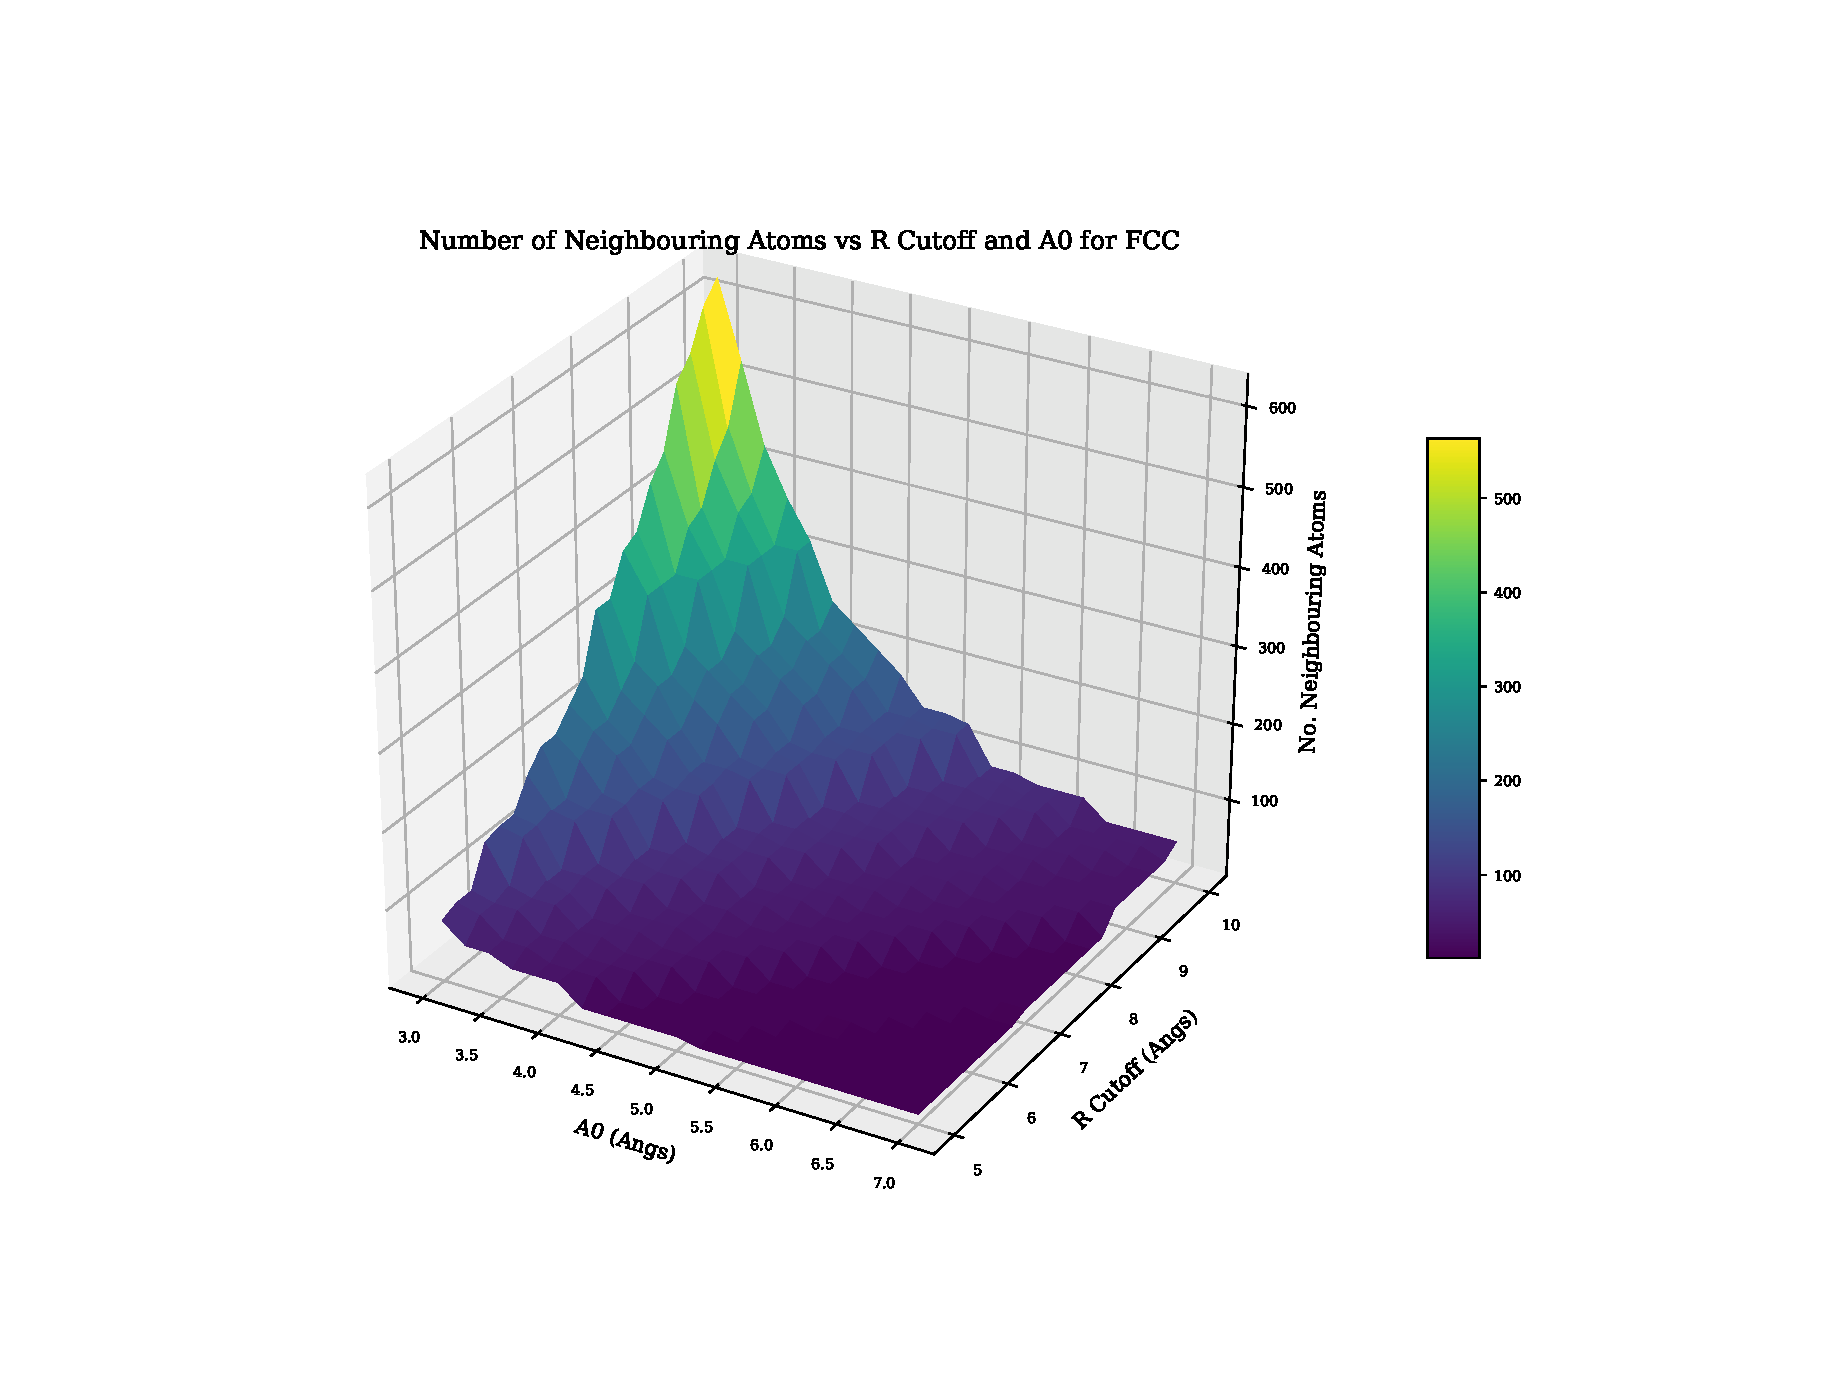
\includegraphics[scale=0.40]{img/atom_neighbours.eps}
    \caption{Graph caption}
    \label{graph:graph1}
  \end{center}
\end{figure}

Building a neighbourlist may take a long while, depending on the parameters.  If a simplistic approach is taken, for N atoms in the supercell, there will be $27N^2$ checks between atoms to see whether they are within the cutoff radius of one another.  For larger numbers of atoms in a supercell, the whole may may be decomposed into smaller domains.

For example, a 16x16x16 FCC supercell, containing 16,384 atoms, would require looping $27 \times 16,384^2 = 7.25 \times 10^9$ times.  Breaking the supercell into 64 smaller domains with 256 atoms in each, reducing the problem to $64 \times 27 \times 256^2 = 1.13 \times 10^8$ loops.

For this program, the supercells used to calculate bulk properties from the interatomic potentials, and the configurations generated by DFT, contain fewer than 1,000 atoms, removing the immediate need add subroutines to decompose the configuration into smaller subcells.

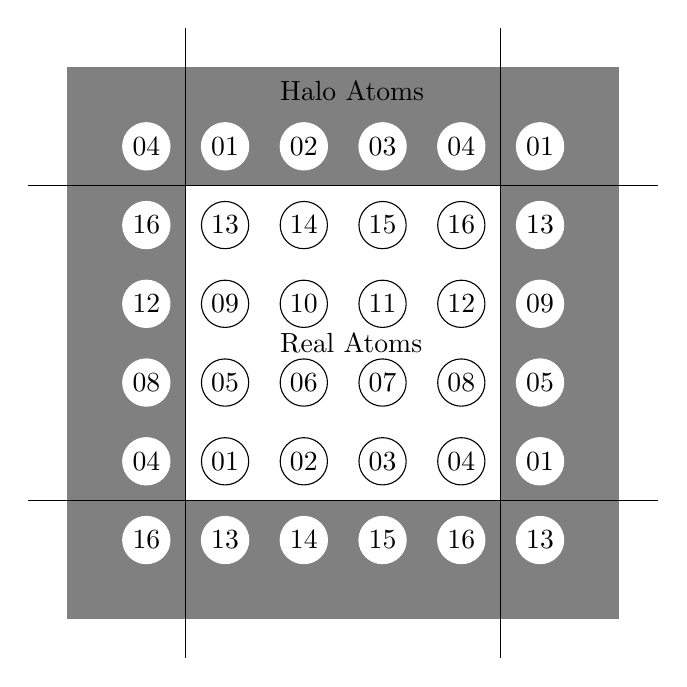
\begin{tikzpicture}
\filldraw [gray] (0.5,0.5) -- (0.5,7.5) -- (7.5,7.5) -- (7.5,0.5) -- (0.5,0.5);
\filldraw [white] (2.0,2.0) -- (2.0,6.0) -- (6.0,6.0) -- (6.0,2.0) -- (2.0,2.0);
\draw (0,2) -- (8,2);
\draw (0,6) -- (8,6);
\draw (2,0) -- (2,8);
\draw (6,0) -- (6,8);
\draw (2.5,2.5) circle [radius=0.3] node {$01$};
\draw (3.5,2.5) circle [radius=0.3] node {$02$};
\draw (4.5,2.5) circle [radius=0.3] node {$03$};
\draw (5.5,2.5) circle [radius=0.3] node {$04$};
\draw (2.5,3.5) circle [radius=0.3] node {$05$};
\draw (3.5,3.5) circle [radius=0.3] node {$06$};
\draw (4.5,3.5) circle [radius=0.3] node {$07$};
\draw (5.5,3.5) circle [radius=0.3] node {$08$};
\draw (2.5,4.5) circle [radius=0.3] node {$09$};
\draw (3.5,4.5) circle [radius=0.3] node {$10$};
\draw (4.5,4.5) circle [radius=0.3] node {$11$};
\draw (5.5,4.5) circle [radius=0.3] node {$12$};
\draw (2.5,5.5) circle [radius=0.3] node {$13$};
\draw (3.5,5.5) circle [radius=0.3] node {$14$};
\draw (4.5,5.5) circle [radius=0.3] node {$15$};
\draw (5.5,5.5) circle [radius=0.3] node {$16$};
\filldraw [white] (1.5,1.5) circle [radius=0.3] node [text=black] {$16$};
\filldraw [white] (1.5,2.5) circle [radius=0.3] node [text=black] {$04$};
\filldraw [white] (1.5,3.5) circle [radius=0.3] node [text=black] {$08$};
\filldraw [white] (1.5,4.5) circle [radius=0.3] node [text=black] {$12$};
\filldraw [white] (1.5,5.5) circle [radius=0.3] node [text=black] {$16$};
\filldraw [white] (1.5,6.5) circle [radius=0.3] node [text=black] {$04$};
\filldraw [white] (2.5,6.5) circle [radius=0.3] node [text=black] {$01$};
\filldraw [white] (3.5,6.5) circle [radius=0.3] node [text=black] {$02$};
\filldraw [white] (4.5,6.5) circle [radius=0.3] node [text=black] {$03$};
\filldraw [white] (5.5,6.5) circle [radius=0.3] node [text=black] {$04$};
\filldraw [white] (6.5,6.5) circle [radius=0.3] node [text=black] {$01$};
\filldraw [white] (6.5,2.5) circle [radius=0.3] node [text=black] {$01$};
\filldraw [white] (6.5,3.5) circle [radius=0.3] node [text=black] {$05$};
\filldraw [white] (6.5,4.5) circle [radius=0.3] node [text=black] {$09$};
\filldraw [white] (6.5,5.5) circle [radius=0.3] node [text=black] {$13$};
\filldraw [white] (6.5,1.5) circle [radius=0.3] node [text=black] {$13$};
\filldraw [white] (2.5,1.5) circle [radius=0.3] node [text=black] {$13$};
\filldraw [white] (3.5,1.5) circle [radius=0.3] node [text=black] {$14$};
\filldraw [white] (4.5,1.5) circle [radius=0.3] node [text=black] {$15$};
\filldraw [white] (5.5,1.5) circle [radius=0.3] node [text=black] {$16$};
\node[text width=3cm] at (4.7,7.2) {Halo Atoms};
\node[text width=3cm] at (4.7,4.0) {Real Atoms};
\end{tikzpicture}



To build the neighbour list a halo configuration is created such that it lies on top of the real atoms, but extends at least as far as the cut off radius on each side of the real simulation box.  Periodic boundary conditions are used to construct the halo.

Once the halo list is computed, the neighbour list may also be computed by looping through the real atoms and halo atoms.  A simple pseudo coded sub routine is given below.


\begin{lstlisting}[style=pseudocode,caption={Simple genetic optimisation subroutine}]

// real_atoms - array holding coordinates of all real atoms
// halo_atoms - array holding coordinates of all halo atoms
// real_ids - unique id for each atom
// halo_ids - unique atom ids for halo atoms
// nlist_ids - array to store ids
// nlist_r - array to store separation

// Define the cutoff and counter start value
r_cut = 5.0
nl_counter = 1

// Calculate square
r_cut_sq = r_cut ** 2

// Loop over all real atoms
DO n_real = 1, real_atom_count
  // Loop over all halo atoms
  DO n_halo = 1, halo_atom_count
    IF (real_ids(n_real) .LT. halo_ids(n_halo)) THEN
      r(1:3) = halo_atoms(n_halo, :) - real_atoms(n_real, :)
      r_sq = SUM(r(1:3) * r(1:3))
      IF (r_sq .LE. r_cut_sq) THEN          
        r_mag = sqrt(r_sq)          
        nlist_ids(nl_counter, 1) = real_ids(n_real)
        nlist_ids(nl_counter, 2) = halo_ids(n_halo)        
        nlist_r(nl_counter, 1) = r_mag
        nlist_r(nl_counter, 2:4) = r(1:3)/r_mag
        nl_counter = nl_counter + 1
      END IF
    END IF
  END DO
END DO 
\end{lstlisting}

The resulting list will contain unique a pair combinations; i.e. the pair atom 1 and atom 2 will only be recorded once, and not also as atom 2 and atom 1.


\subsubsection{Computing Total Energy}

The total energy of the system is the sum of the individual energies for the atoms in the simulation.  The type of atom (or pairs of atoms) will determine which function is used.

First, to compute the pair potentials:

\begin{itemize}
\item set the total energy of the system equal to zero
\item set the starting energy for each atom in the system to zero
\item loop through the atom pairs in the entire neighbour list
\item for each atom pair, A and B, use the known separation and the potential function to compute the potential energy on atom A due to B and vice versa
\item add this potential energy to both A and B
\item after looping through the neighbour list, add all the energies due to the pair potential to the total energy
\end{itemize}

For an EAM or 2BEAM potential, the densities and embedding energies must also be computed:

\begin{itemize}
\item set the electron density at the position of (for each) atom to zero
\item loop through the atom pairs in the entire neighbour list
\item for each atom pair, using the density function for the atom A, the density at atom B due to atom A will be calculated and added to the density at atom B
\item if the atoms are both of the same type the same density will be added to atom A due to atom B
\item if the atom types are different, using the density function for the atom B, the density at atom A due to atom B will be calculated and added to the density at atom A
\item following looping through the neighbour list, to calculate the densities at each atom, the list of atoms will be looped through
\item for each atom, the density value at the position of that atom, will be input into the appropriate embedding function to calculate the embedding portion of the energy
\item add all the embedding energies to the total energy of the system
\end{itemize}

For a 2BEAM potential, repeat the above procedure for the second group of density functions and embedding functions (do not repeat calculation of the pair potentials).


\subsubsection{Computing Forces on Atoms}

In order to calculate the forces on the atoms with an EAM or 2 Band EAM potential, the neighbour list and atom list will need to be looped through several times.  First, the pair potential and force due to the pair potential must be calculated by a complete loop through the neighbour list.  At the same time, the density at each atom location is also calculated.  The embedding energy may then be computed by looping through all the atoms and using the electron density at each atom to give the energy of the atom embedded in that density.  The third and final loop will run through the neighbour pairs in the neighbour list once more computing the force on each atom due to it's embedding.


\subsubsection{Computing Forces on Atoms}

\subsubsection{Pseudo Code for the Energy, Force and Stress Subroutine}

\begin{lstlisting}[style=pseudocode,caption={Pseudo Code for Energy and Stress Force Calculation}]

electron_density[1:n_atoms, 1:bands] = 0.0  // electron density at each atom
density_grad_ab[:,:] = 0.0                  // grad density function
density_grad_ba[:,:] = 0.0                  // grad density function
energy = 0.0                                // total energy
forces[:,:] = 0.0                           // forces each atom, 3D
force_between_pairs[:,:] = 0.0              // used to store force between pairs, for stress computation
stress[:,:] = 0.0D0

// LOOP 1 - Pair energy, force and calculate densities
DO n = 1, neighbour_count
  E = get_PairEnergy(atom_a, atom_b, r[n,:])
  F[:] = get_PairForce(atom_a, atom_b, r[n,:])

  // Save energy
  energy = energy + E

  // Save Force
  f[atom_a, :] = f[atom_a, :] - F[:]
  f[atom_b, :] = f[atom_b, :] + F[:]
  force_between_pairs[:,:] = force_between_pairs[:,:] - F[:]   // Used to calculate stress
  
  // Loop through density bands
  DO band = 1, bands
    // Electron density at A due to atom B
    electron_density[atom_a, b] = get_Density(atom_b, r)
    density_grad_ab[n, band] = get_DensityGradient(atom_b, r)
  
    // Electron density at B due to atom A
    electron_density[atom_a, band] = get_Density(atom_a, r)
    density_grad_ba[n, band] = get_DensityGradient(atom_a, r)
  END DO
END DO

// LOOP 2 - Embedding energy
DO n = 1, atom_count
  // Loop through density bands
  DO band = 1, bands
    energy = energy + get_EmbeddingEnergy(n, band)
  END DO
END DO

// LOOP 3 - Embedding force
DO n = 1, neighbour_count
  // Loop through density bands
  DO band = 1, bands
    epA = get_EmbeddingGradient(atom_a, electron_density(atom_a, b))
    epB = get_EmbeddingGradient(atom_b, electron_density(atom_b, b))

    F[:] = (epA * density_grad_ba(n, band) + epB * density_grad_ab(n, band)) * r[n, :]

    f[atom_a, :) = f(atom_a, :) - F[:] 
    f(atom_a, :) = f(atom_a, :) + F[:] 
    
    force_between_pairs[:,:] = force_between_pairs[:,:] - F[:]   // Used to calculate stress
  END DO
END DO

// LOOP 4 STRESS
DO n = 1, neighbour_count
  // Only compute if the second atom is in the halo 
  IF(nlisthalo(n))THEN  
    DO i = 1,3
      DO j = 1,3
        stress[i,j] = stress[i,j] + (r[n, i] * force_between_pairs[n,j])
      END DO
    END DO
  END IF
END DO
stress[1:3, 1:3] = stress[1:3, 1:3] / (2.0 * volume)

\end{lstlisting}






\section{Equation of State for Cubic Crystals}

\subsection{Murnaghan Equation of State}

Hooke's law implies a linear relationship between stress and strain.  In practice, where a pressure is applied to a material, the application of Hooke's law is limited \cite{murnaghaneq}.  Muraghan derived a new equation to improve upon formulae developed in the 1930's, using compression data from high pressure experiments.

\begin{equation}
\begin{split}
P(V) = \frac{B_0}{{B'}_0}\left(\left(\frac{V_0}{V}\right)^{{B'}_0}-1\right)
\end{split}
\label{eq:eqMurnachanEquationofStatePressure}
\end{equation}

As pressure is the negative derivative of the internal energy of the system with respect to change in volume, $p = -(\partial E/dV)$, and the equation can be integrated and written in terms of the energy, volume, bulk modulus and its derivative\cite{crystaleos}.

\begin{equation}
\begin{split}
E(V) = E_0 + \frac{B_0 V}{{B'}_0} \left[\left(\frac{V_0}{V}\right)^{{B'}_0} \frac{1}{{B'}_0 - 1} + 1 \right] - \frac{B_0 V_0}{{B'}_0-1}
\end{split}
\label{eq:eqMurnachanEquationofStateEnergy}
\end{equation}

\subsection{Birch-Murnaghan Equation of State}

Several years after Murnaghan's equation, Birch developed further upon the experimental data provided by Bridgman.  For cubic symmetry, the description of free energy now includes third order terms in the strain components\cite{birchmurnaghaneq}.

\begin{equation}
\begin{split}
P(V) = \frac{3 B_0}{2} \left[\left(\frac{V_0}{V}\right)^{\frac{7}{3}}-\left(\frac{V_0}{V}\right)^{\frac{5}{3}}\right] \left[1 + \frac{3}{4}({B'}_0-4)\left(\left(\frac{V_0}{V}\right)^{\frac{2}{3}}-1\right)\right]
\end{split}
\label{eq:eqMurnachan Equation of State}
\end{equation}

The energy-volume relationship may again be constructed\cite{crystaleos}.

\begin{equation}
\begin{split}
E(V) = E_0 + \frac{9 V_0 B_0}{16} \left[ \left[ \left(\frac{V_0}{V} \right)^{\frac{2}{3}}-1\right]^{3} {B'}_0 + \left[ \left(\frac{V_0}{V} \right)^{\frac{2}{3}}-1\right]^{2} \left[6 - 4 \left(\frac{V_0}{V} \right)^{\frac{2}{3}}\right] \right]
\end{split}
\label{eq:eqMurnachanEquationofStateVolume}
\end{equation}



\subsection{Fitting Method}

The first step is to fit a second order polynomial to the energy-volume data.  This may be achieved using least-squares fitting with a vandermode matrix.  The coefficients from this polynomial may then be used to calculate reasonable value for $E_0$, $V_0$ and $B_0$; sane starting values of ${B'}_0$ are between 1 and 10, and the code takes a starting value of 2\cite{gilgamesheos}.

\begin{equation}
\begin{split}
E(V) = c_0 + c_1 V + c_2 V^2 \\
V_0 = -\frac{c_1}{2c_2} \\
E_0 = c_2 * {V_0}^2 + c_1 V_0 + c_0  \\
B_0 = 2 c_2 V_0 \\
{B'}_0 = 2
\end{split}
\label{eq:eqMurnachanEquationofStateVolume}
\end{equation}

Newton Gauss is then used to minimise $E_0$, $V_0$ and $B_0$ while ${B'}_0 \in {1.0,1.5,2.0,2.5,3.0,3.5,4.0,4.5,5.0,5.5,6.0}$

\begin{equation}
\begin{split}
\left[J^T J\right] P = J^T R
\end{split}
\label{eq:eqMurnachanEquationofStateVolume}
\end{equation}

The parameters with the lowest residual square sum are returned.







\subsection{Calculating Elastic Constants for Orthorhombic Crystal}


The DFT work here includes Palladium and Iron.  The natural arrangement of Pd atoms in a pure sample are FCC within a cubic crystal.  Pure iron at room temperature is BCC, but this work is interested in austenetic stainless steel where the structure of atoms in the alloy are FCC.  When modelling FCC iron using DFT with a non-polarized calculation, the crystal favours a cubic crystal with the atoms fixed in the FCC positions.  When a spin-polarized calculation is computed, with magnetization along the x-axis, the crystal becomes tetragonal (once again, the atoms are fixed in FCC positions).


\begin{center}
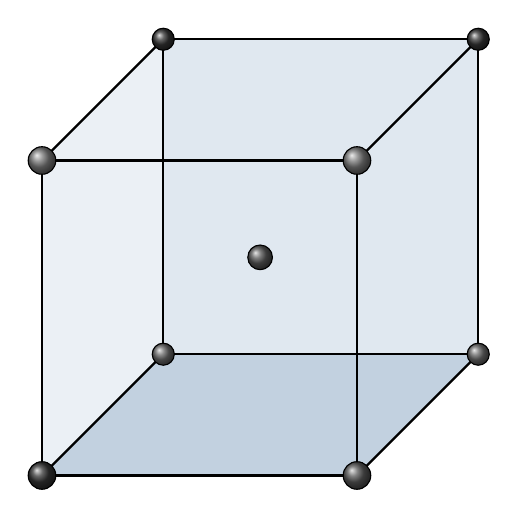
\begin{tikzpicture}[scale=0.5]
\fill[col_336699!10,opacity=1.0] (0.0,0.0,0.0) -- (0.0,0.0,8.0) -- (0.0,8.0,8.0) -- (0.0,8.0,0.0) -- cycle;     %% bottom square
\fill[col_336699!15,opacity=1.0] (0.0,0.0,0.0) -- (0.0,8.0,0.0) -- (8.0,8.0,0.0) -- (8.0,0.0,0.0) -- cycle;     %% bottom square
\fill[col_336699!30,opacity=1.0] (0.0,0.0,0.0) -- (8.0,0.0,0.0) -- (8.0,0.0,8.0) -- (0.0,0.0,8.0) -- cycle;     %% bottom square
\draw[solid, col_000000, thick] (0.0,0.0,8.0) -- (0.0,0.0,0.0); 
\draw[solid, col_000000, thick] (0.0,0.0,0.0) -- (0.0,8.0,0.0); 
\draw[solid, col_000000, thick] (0.0,0.0,0.0) -- (8.0,0.0,0.0); 
\draw[solid, col_000000, thick] (0.0,8.0,8.0) -- (0.0,8.0,0.0); 
\draw[solid, col_000000, thick] (0.0,8.0,0.0) -- (8.0,8.0,0.0); 
\draw[solid, col_000000, thick] (8.0,0.0,8.0) -- (8.0,0.0,0.0); 
\draw[solid, col_000000, thick] (8.0,0.0,0.0) -- (8.0,8.0,0.0); 
\draw[solid, col_000000, thick] (8.0,8.0,8.0) -- (8.0,8.0,0.0); 
\tikzdrawatom{col_666666}{0.0}{0.0}{0.0}{0.27999999999999997} 
\tikzdrawatom{col_333333}{0.0}{8.0}{0.0}{0.27999999999999997} 
\tikzdrawatom{col_666666}{8.0}{0.0}{0.0}{0.27999999999999997} 
\tikzdrawatom{col_333333}{8.0}{8.0}{0.0}{0.27999999999999997} 
\tikzdrawatom{col_555555}{4.0}{4.0}{4.0}{0.3130495168499705} 
\draw[solid, col_000000, thick] (0.0,0.0,8.0) -- (0.0,8.0,8.0); 
\draw[solid, col_000000, thick] (0.0,0.0,8.0) -- (8.0,0.0,8.0); 
\draw[solid, col_000000, thick] (0.0,8.0,8.0) -- (8.0,8.0,8.0); 
\draw[solid, col_000000, thick] (8.0,0.0,8.0) -- (8.0,8.0,8.0); 
\tikzdrawatom{col_333333}{0.0}{0.0}{8.0}{0.35} 
\tikzdrawatom{col_777777}{0.0}{8.0}{8.0}{0.35} 
\tikzdrawatom{col_555555}{8.0}{0.0}{8.0}{0.35} 
\tikzdrawatom{col_777777}{8.0}{8.0}{8.0}{0.35} 
\end{tikzpicture} 

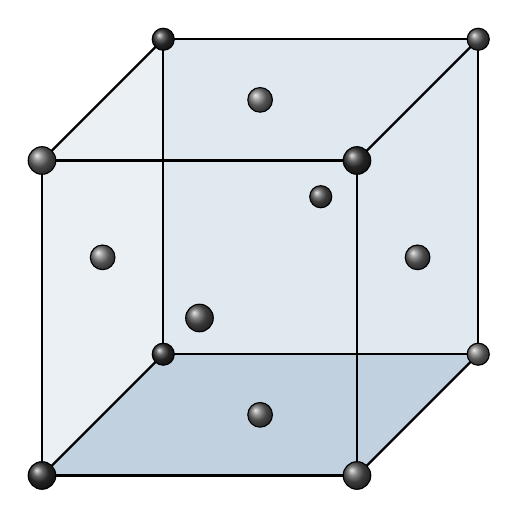
\begin{tikzpicture}[scale=0.5]
\fill[col_336699!10,opacity=1.0] (0.0,0.0,0.0) -- (0.0,0.0,8.0) -- (0.0,8.0,8.0) -- (0.0,8.0,0.0) -- cycle;     %% bottom square
\fill[col_336699!15,opacity=1.0] (0.0,0.0,0.0) -- (0.0,8.0,0.0) -- (8.0,8.0,0.0) -- (8.0,0.0,0.0) -- cycle;     %% bottom square
\fill[col_336699!30,opacity=1.0] (0.0,0.0,0.0) -- (8.0,0.0,0.0) -- (8.0,0.0,8.0) -- (0.0,0.0,8.0) -- cycle;     %% bottom square
\draw[solid, col_000000, thick] (0.0,0.0,8.0) -- (0.0,0.0,0.0); 
\draw[solid, col_000000, thick] (0.0,0.0,0.0) -- (0.0,8.0,0.0); 
\draw[solid, col_000000, thick] (0.0,0.0,0.0) -- (8.0,0.0,0.0); 
\draw[solid, col_000000, thick] (0.0,8.0,8.0) -- (0.0,8.0,0.0); 
\draw[solid, col_000000, thick] (0.0,8.0,0.0) -- (8.0,8.0,0.0); 
\draw[solid, col_000000, thick] (8.0,0.0,8.0) -- (8.0,0.0,0.0); 
\draw[solid, col_000000, thick] (8.0,0.0,0.0) -- (8.0,8.0,0.0); 
\draw[solid, col_000000, thick] (8.0,8.0,8.0) -- (8.0,8.0,0.0); 
\tikzdrawatom{col_333333}{0.0}{0.0}{0.0}{0.27999999999999997} 
\tikzdrawatom{col_555555}{4.0}{4.0}{0.0}{0.27999999999999997} 
\tikzdrawatom{col_333333}{0.0}{8.0}{0.0}{0.27999999999999997} 
\tikzdrawatom{col_777777}{8.0}{0.0}{0.0}{0.27999999999999997} 
\tikzdrawatom{col_555555}{8.0}{8.0}{0.0}{0.27999999999999997} 
\tikzdrawatom{col_666666}{4.0}{0.0}{4.0}{0.3130495168499705} 
\tikzdrawatom{col_777777}{0.0}{4.0}{4.0}{0.3130495168499705} 
\tikzdrawatom{col_777777}{4.0}{8.0}{4.0}{0.3130495168499705} 
\tikzdrawatom{col_666666}{8.0}{4.0}{4.0}{0.3130495168499705} 
\draw[solid, col_000000, thick] (0.0,0.0,8.0) -- (0.0,8.0,8.0); 
\draw[solid, col_000000, thick] (0.0,0.0,8.0) -- (8.0,0.0,8.0); 
\draw[solid, col_000000, thick] (0.0,8.0,8.0) -- (8.0,8.0,8.0); 
\draw[solid, col_000000, thick] (8.0,0.0,8.0) -- (8.0,8.0,8.0); 
\tikzdrawatom{col_333333}{0.0}{0.0}{8.0}{0.35} 
\tikzdrawatom{col_555555}{4.0}{4.0}{8.0}{0.35} 
\tikzdrawatom{col_666666}{0.0}{8.0}{8.0}{0.35} 
\tikzdrawatom{col_555555}{8.0}{0.0}{8.0}{0.35} 
\tikzdrawatom{col_333333}{8.0}{8.0}{8.0}{0.35} 
\end{tikzpicture} 
\end{center}




\begin{equation}
    \begin{split}
      C_{ij} = 
      \begin{bmatrix}
      C_{11} & C_{12} & C_{13} & 0      & 0      & 0      \\
      C_{12} & C_{22} & C_{23} & 0      & 0      & 0      \\
      C_{13} & C_{23} & C_{33} & 0      & 0      & 0      \\
      0      & 0      & 0      & C_{44} & 0      & 0      \\
      0      & 0      & 0      & 0      & C_{55} & 0      \\
      0      & 0      & 0      & 0      & 0      & C_{66} \\
      \end{bmatrix}\\
      \text{(9 independent values)}
    \end{split}
    \label{eq:eqOrthoRhombicEC}
\end{equation}







Once the optimised parameters have been determined for the orthorhombic crystal, nine strains are applied to the crystal \cite{DftTiSiRavindran} in order to calculate the nine independent elastic constants.

  \begin{equation}
    \begin{split}
    E(V,\sigma) = E(V_{0},0) + V_{0} \left( \sum_{i} \tau_i \epsilon_i \sigma_i + \frac{1}{2} \sum_{ij} c_{ij} \sigma_{i} \epsilon{i} \sigma_{j} \epsilon{j} \right) + O(\sigma^3)
    \end{split}
  \end{equation}

The first three strains applied to the orthorhombic crystal 

\begin{equation}
    \begin{split}
      D_{1} = 
      \begin{bmatrix}
      1 + \delta & 0       & 0             \\
      0          & 1       & 0             \\
      0          & 0       & 1             \\
      \end{bmatrix}
    \end{split}
\end{equation}

  \begin{equation}
    \begin{split}
    E(V,\sigma) = E(V_{0},0) + V_{0} \left( \tau_{1} \sigma + \frac{c_{11}}{2} \sigma^2 \right)
    \end{split}
  \end{equation}


  \begin{equation}
    \begin{split}
      D_{2} = 
      \begin{bmatrix}
      1          & 0           & 0             \\
      0          & 1 + \delta  & 0             \\
      0          & 0           & 1             \\
      \end{bmatrix}
    \end{split}
  \end{equation}

  \begin{equation}
    \begin{split}
    E(V,\sigma) = E(V_{0},0) + V_{0} \left( \tau_{2} \sigma + \frac{c_{22}}{2} \sigma^2 \right)
    \end{split}
  \end{equation}



  \begin{equation}
    \begin{split}
      D_{3} = 
      \begin{bmatrix}
      1          & 0           & 0             \\
      0          & 1           & 0             \\
      0          & 0           & 1 + \delta    \\
      \end{bmatrix}
    \end{split}
  \end{equation}

  \begin{equation}
    \begin{split}
    E(V,\sigma) = E(V_{0},0) + V_{0} \left( \tau_{3} \sigma + \frac{c_{33}}{2} \sigma^2 \right)
    \end{split}
  \end{equation}


Volume conserving monoclinic distortions are then applied to the crystal to calculate the $C_11$, $C_22$ and $C_33$ elastic constants.

  \begin{equation}
    \begin{split}
      D_{4} = 
      \begin{bmatrix}
      \frac{1}{(1-\sigma^2)^{\frac{1}{3}}} & 0           & 0             \\
      0                                    & \frac{1}{(1-\sigma^2)^{\frac{1}{3}}}      & \frac{\sigma}{(1-\sigma^2)^{\frac{1}{3}}}  \\
      0                                    & \frac{\sigma}{(1-\sigma^2)^{\frac{1}{3}}} & \frac{1}{(1-\sigma^2)^{\frac{1}{3}}}       \\
      \end{bmatrix}
    \end{split}
  \end{equation}

  \begin{equation}
    \begin{split}
    E(V,\sigma) = E(V_{0},0) + V_{0} \left(2 \tau_{4} \sigma + 2 \frac{c_{44}}{2} \sigma^2 \right)
    \end{split}
  \end{equation}

  \begin{equation}
    \begin{split}
      D_{5} = 
      \begin{bmatrix}
      \frac{1}{(1-\sigma^2)^{\frac{1}{3}}} & 0           & \frac{\sigma}{(1-\sigma^2)^{\frac{1}{3}}}              \\
      0                                    & \frac{1}{(1-\sigma^2)^{\frac{1}{3}}}      &   0  \\
      \frac{\sigma}{(1-\sigma^2)^{\frac{1}{3}}}   &   0  & \frac{1}{(1-\sigma^2)^{\frac{1}{3}}}       \\
      \end{bmatrix}
    \end{split}
  \end{equation}

  \begin{equation}
    \begin{split}
    E(V,\sigma) = E(V_{0},0) + V_{0} \left(2 \tau_{5} \sigma + 2 \frac{c_{55}}{2} \sigma^2 \right)
    \end{split}
  \end{equation}



  \begin{equation}
    \begin{split}
      D_{6} = 
      \begin{bmatrix}
      \frac{1}{(1-\sigma^2)^{\frac{1}{3}}}        & \frac{\sigma}{(1-\sigma^2)^{\frac{1}{3}}} & 0   \\
      \frac{\sigma}{(1-\sigma^2)^{\frac{1}{3}}}   & \frac{1}{(1-\sigma^2)^{\frac{1}{3}}}      &   0  \\
      0                                           & 0                                         & \frac{1}{(1-\sigma^2)^{\frac{1}{3}}}       \\
      \end{bmatrix}
    \end{split}
  \end{equation}

  \begin{equation}
    \begin{split}
    E(V,\sigma) = E(V_{0},0) + V_{0} \left(2 \tau_{6} \sigma + 2 \frac{c_{66}}{2} \sigma^2 \right)
    \end{split}
  \end{equation}



  \begin{equation}
    \begin{split}
      D_{7} = 
      \begin{bmatrix}
      \frac{1 + \sigma}{(1-\sigma^2)^{\frac{1}{3}}} & 0           & 0              \\
      0                                    & \frac{1 - \sigma}{(1-\sigma^2)^{\frac{1}{3}}}      &   0  \\
      0  &   0  & \frac{1}{(1-\sigma^2)^{\frac{1}{3}}}       \\
      \end{bmatrix}
    \end{split}
  \end{equation}

  \begin{equation}
    \begin{split}
    E(V,\sigma) = E(V_{0},0) + V_{0} \left((\tau_{1}-\tau{2} \sigma + \frac{1}{2} (c_{11} + c_{22} - 2 c{12}) \sigma^2 \right)
    \end{split}
  \end{equation}


  \begin{equation}
    \begin{split}
      D_{8} = 
      \begin{bmatrix}
      \frac{1 + \sigma}{(1-\sigma^2)^{\frac{1}{3}}} & 0           & 0              \\
      0                                    & \frac{1}{(1-\sigma^2)^{\frac{1}{3}}}      &   0  \\
      0  &   0  & \frac{1-\sigma}{(1-\sigma^2)^{\frac{1}{3}}}       \\
      \end{bmatrix}
    \end{split}
  \end{equation}

  \begin{equation}
    \begin{split}
    E(V,\sigma) = E(V_{0},0) + V_{0} \left((\tau_{1}-\tau{3} \sigma + \frac{1}{2} (c_{11} + c_{33} - 2 c{13}) \sigma^2 \right)
    \end{split}
  \end{equation}


  \begin{equation}
    \begin{split}
      D_{9} = 
      \begin{bmatrix}
      \frac{1}{(1-\sigma^2)^{\frac{1}{3}}} & 0           & 0              \\
      0  & \frac{1 + \sigma}{(1-\sigma^2)^{\frac{1}{3}}}      &   0  \\
      0  &   0  & \frac{1 - \sigma}{(1-\sigma^2)^{\frac{1}{3}}}       \\
      \end{bmatrix}
    \end{split}
  \end{equation}

  \begin{equation}
    \begin{split}
    E(V,\sigma) = E(V_{0},0) + V_{0} \left((\tau_{2}-\tau{3} \sigma + \frac{1}{2} (c_{22} + c_{33} - 2 c{23}) \sigma^2 \right)
    \end{split}
  \end{equation}


\subsection{Elastic Constants: Bulk Modulus, Young's Modulus, Shear Modulus and Poisson Ratio}

The bulk modulus, as noted earlier, is a measure of the effect of strain on stress.  While it may be calculated by taking the second derivative of energu with respect to volume, or by fitting an equation of state, it may also be calculated using the elastic constants of a material or the compliance constants.

The Young's modulus is a measure of the stiffness of a material, and the shear modulus (also know as the modulus of rigidity) 

\begin{equation}
\begin{split}
B_{V} = \frac{1}{9} \left( C_{11} + C_{22} + C_{33} + 2(C_{12} + C_{13} + C_{23}) \right)
\end{split}
\label{eq:eqLennardJones}
\end{equation}

\begin{equation}
\begin{split}
B_{R} = \left( S_{11} + S_{22} + S_{33} + 2(S_{12} + S_{13} + S_{23}) \right)^{-1}
\end{split}
\label{eq:eqLennardJones}
\end{equation}






\section{Force Matching}

To derive a potential, one may approach the problem from first principles in an attempt to replicate reality.  It has been more useful, however, to lose any physical elegance \cite{twobandackland} to give potentials that work for specific elements under certain conditions.  Force data, gathered experimentally or by first-principles calculations, has been used to develop potentials since the 1990s.  The force matching method was developed in 1994 by Ercolessi and Adams \cite{forcematchingmethod} to link the more accurate, more processor and memory intensive, world of first-principles calculations to Molecular Dynamics.

The force-matching method uses the difference between the actual force (either measured experimentally or calculated by first-principles calculations) 

Given a set of M different atomic configurations, and a potential with a set of L parameters ($ \vec{p} $), the function $Z_F$ is a measure of the difference between the the forces calculated using the potential for all configurations and the actual (or DFT generated) forces.

\begin{equation}
\begin{split}
Z_F(\vec{\alpha}) = \sum _{k=1}^M \sum _{i=1} ^{k} \sum _{j=1} ^{3} \lvert \vec{F^k_{i,j} (\vec{\alpha})} - \vec{F^0_{i,j}} \rvert^2
\end{split}
\label{eq:eqForceMatchingB}
\end{equation}

This may be extended to include the calculation of other properties, including the cohesive energy of atoms, the lattice parameter, bulk modulus, elastic constants and so on.  Each may be weighted depending on how important the property is to the simulation the potential is required for.

\begin{equation}
\begin{split}
Z(\vec{p}) = w_{F} Z_F(\vec{p}) + w_{b0} Z_{b0}(\vec{p}) + w_{e0} Z_{e0}(\vec{p}) + w_{a0} Z_{a0}(\vec{p}) + w_{ec} Z_{ec}(\vec{p}) + w_{ecoh} Z_{ecoh}(\vec{p})
\end{split}
\label{eq:eqForceMatchingA}
\end{equation}




\section{D-Band and S-Band}

\subsection{Finnis-Sinclair Potential with S and D Band Contributions}

The transition element, Caesium, has a the electron configuration [Xe] $6s^1$.  The single valence electron in the 6s shell can be promoted to the higher energy and more compact 6d shell under compression, reducing the atom's size.  The bond energy may be calculated from the energies of each band plus the energy required to promote from one band to the other\cite{twobandacklandreed}.


\begin{equation}
\begin{split}
U_{bond} = \sum_{i} \frac{w_{i,1}}{nN_1} n_{i1}(n_{i1}-N_1) + \sum_{i} \frac{w_{i2}}{2N_2} n_{i1} (n_{i2} - N_{2}) + E_{prom} \\
N_1, N_2 \text{capacities of each band} \\
n_{i1}, n_{i2} \text{electrons in each band of} i^{th} \text{atom} \\
E_{prom} = \text{Energy required to promote electron from band 1 to 2}
\end{split}
\label{eq:eq2BandBondEnergy}
\end{equation}

A Finnis-Sinclair potential was derived for Caesium by Ackland and Reed.

The pair functions are defined as:

\begin{equation}
\begin{split}
V_s (r_{ij}) = \sum_j \frac{A_s}{{r_{ij}}^{12}} \\
V_d (r_{ij}) = \sum_j \frac{A_d}{{r_{ij}}^{12}}
\end{split}
\label{eq:caseiumPairFunction}
\end{equation}


For the s-band electron density:

\begin{equation}
\begin{split}
\phi_{s} (r_{ij}) =% 
\begin{cases}
C_s \left(d_s-r_{ij}\right)^3 & r_{ij} <= d_s \\
0 & r_{ij} > d_s
\end{cases}
\end{split}
\label{eq:caesiumDensityS}
\end{equation}

For the d-band electron density:

\begin{equation}
\begin{split}
\phi_{d} (r_{ij}) =% 
\begin{cases}
C_d \left(d_d-r_{ij}\right)^3 & r_{ij} <= d_d \\
0 & r_{ij} > d_d
\end{cases}
\end{split}
\label{eq:caesiumDensityD}
\end{equation}

The embedding function is the standard Finnis-Sinclair embedding function:

\begin{equation}
\begin{split}
F(\rho) = \sqrt{\rho}
\end{split}
\label{eq:finnisSinclairEmbedding}
\end{equation}

As pressure is applied to Caesium, it changes several times.

\begin{center}
I     Cs BCC at ambient pressure (115.9 angstrom cubed per atom) \\
$\downarrow$ \\
II    Cs FCC with slight pressure (67.5 angstrom cubed per atom) \\
$\downarrow$ \\
III   Cs FCC isostructural transformation (48.7 angstrom cubed per atom)
\end{center}

The parameters derived by Ackland and Reed were "in good agreement with experiment" with the 4.3GPa transition pressure between Cs II and Cs III.


\subsection{Density and Embedding Groups}

This program may be use potentials with just one density and embedding function per element.  It may also be configured to use two or more groups of densities and embedding energies per element; for example s-band and d-band electrons.



\begin{equation}
\begin{split}
U_{EAM} = V_{pair} + \sum_{b}^B F_b (\rho_b)
\frac{1}{2} \sum \limits_{i=1}^{N} \sum \limits_{j\ne i}^{N} V_{ij}(r_{ij}) + \sum \limits_{b=1}^{B} \sum \limits_{i=1}^{N} F_{b}[\rho _{b,i}]
\textnormal{where   } \rho_{b,i} = \sum \limits_{j=i,j \ne i}^{N} \rho_{b,ij}(r_{ij})
\textnormal{and B total number of bands, 1, 2, 3 etc}
\end{split}
\end{equation}






%%######################################################################
%% Installation
%%######################################################################


\chapter{Installation}

\section{Requirements}

The program was written to work with the following:

\begin{itemize}
\item Linux Debian
\item Fortran with OpenMP
\item Python 3
\end{itemize}


The program takes advantage of multicore processors.  The amount of RAM needed by a calculation is specified in the configuration file.  Several gigabyte should be enough.



\section{How To Install}

\begin{lstlisting}
sudo apt install gfortran libomp-dev
sudo apt install python3 python3-matplotlib python3-numpy python3-tk

cd ~/
mkdir eampa && cd ~/eampa
git clone https://github.com/BenPalmer1983/eampa_v3
cd eampa_v3
cd f2py_src
./build.sh
\end{lstlisting}






%%######################################################################
%% How to Use
%%######################################################################


\chapter{How To Use}


\section{Set Up Working Directory}




\section{}




%%######################################################################
%% Appendix
%%######################################################################



\begin{appendices}




\chapter{Functions}

\section{Introduction}

This section of the appendix covers the types of potential function and common choices of function used and details on how to use these in the potential fitting code.


\section{Pair Functions}

\subsection{Lennard-Jones}

\begin{figure}[h]
  \begin{center}
    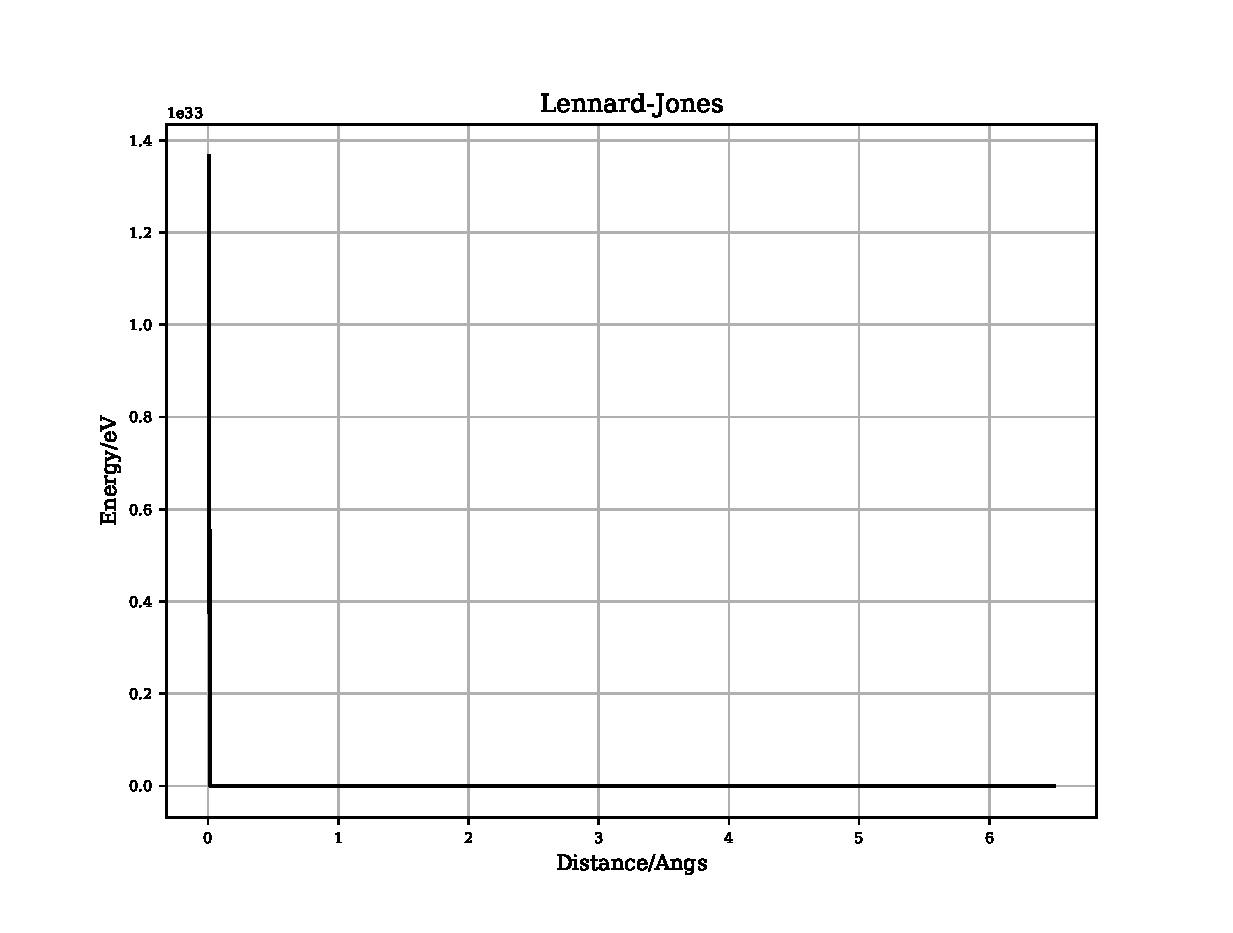
\includegraphics{img/plots/lennard_jones.eps}[scale=0.6]
    \caption{Lennard-Jones}
    \label{graph:graph1}
  \end{center}
\end{figure}

\begin{equation}
\begin{split}
V(r) = e \left(\left(\frac{r_m}{r}\right)^12 - 2 \left(\frac{r_m}{r}\right)^6\right)
\end{split}
\label{eq:eqLennardJones}
\end{equation}

\begin{lstlisting}[style=pseudocode,caption={Lennard-Jones}]
#A
#TYPE lennard_jones
#P 2.3 3.5
#L 0.0
#U 7.0
\end{lstlisting}






\subsection{Morse}

\begin{figure}[h]
  \begin{center}
    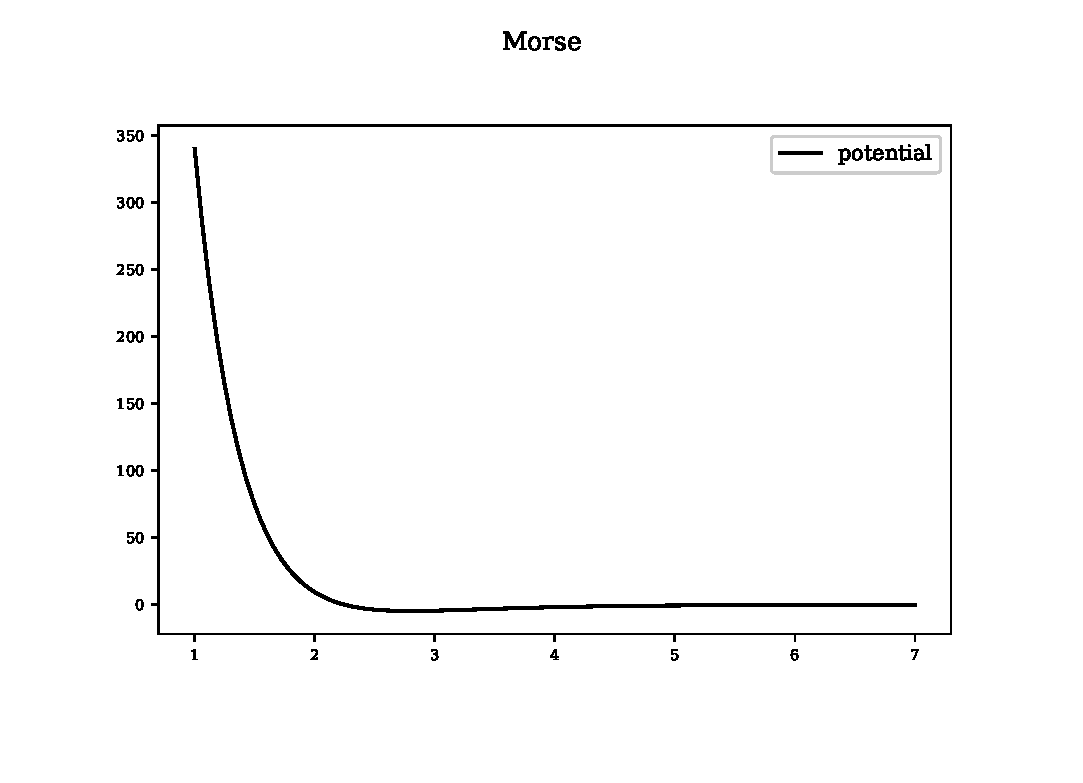
\includegraphics{img/plots/morse.eps}[scale=0.6]
    \caption{Morse}
    \label{graph:graph1}
  \end{center}
\end{figure}

\begin{equation}
\begin{split}
V(r) = exp(-2 a (r - re)) - 2 exp (-a*(r - re))
\end{split}
\label{eq:eqMorse}
\end{equation}

\begin{lstlisting}[style=pseudocode,caption={Morse}]
#A
#TYPE morse
#P 4.669 1.256 2.8
#L 0.0
#U 7.0
\end{lstlisting}





\subsection{Buckingham}

\begin{figure}[h]
  \begin{center}
    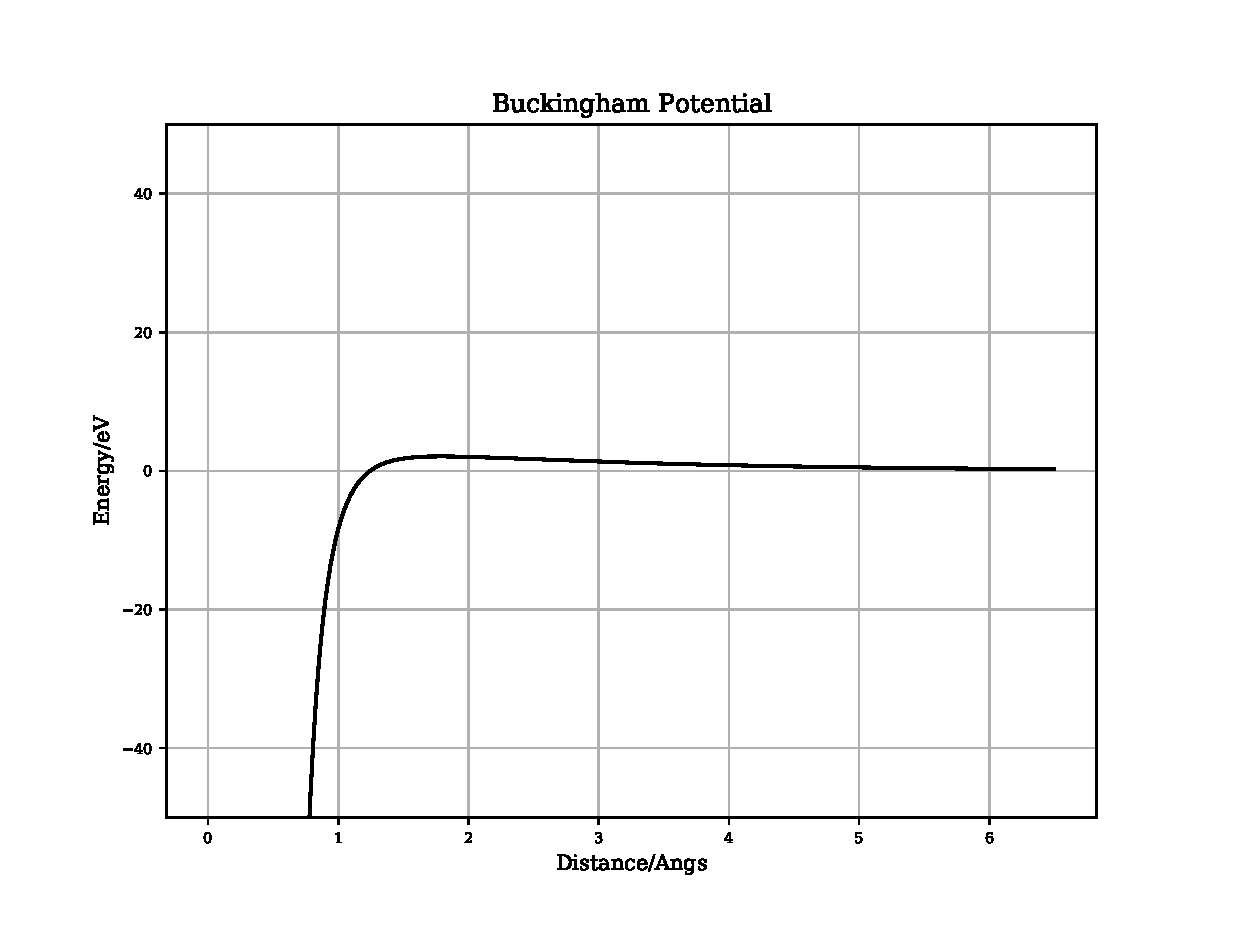
\includegraphics{img/plots/buckingham.eps}[scale=0.6]
    \caption{Buckingham}
    \label{graph:graph1}
  \end{center}
\end{figure}

\begin{equation}
\begin{split}
V(r) = A * exp(-B * r) - \frac{C}{r**6}
\end{split}
\label{eq:eqBuckingham}
\end{equation}

\begin{lstlisting}[style=pseudocode,caption={Buckingham}]
#A
#TYPE buckingham
#P 6.0 0.5 12.0
#L 0.0
#U 7.0
\end{lstlisting}





\subsection{ZBL}

\begin{equation}
\begin{split}
\phi(x) = 0.181 e^{-3.2x} + 0.5099 e^{-0.9423x} + 0.2802 e^{-0.4029x} + 0.02817 e^{-0.2016x} \\
\text{where } a_{ij} = \frac{0.8854 a_0}{Z^{0.23}_i + Z^{0.23}_j} \\
\text{and } a_0 = 0.529 \text{angstrom}
\end{split}
\label{eq:screeningPotential}
\end{equation}






\subsection{Quartic Polynomial Plus Exponential Repulsion}

\begin{figure}[h]
  \begin{center}
    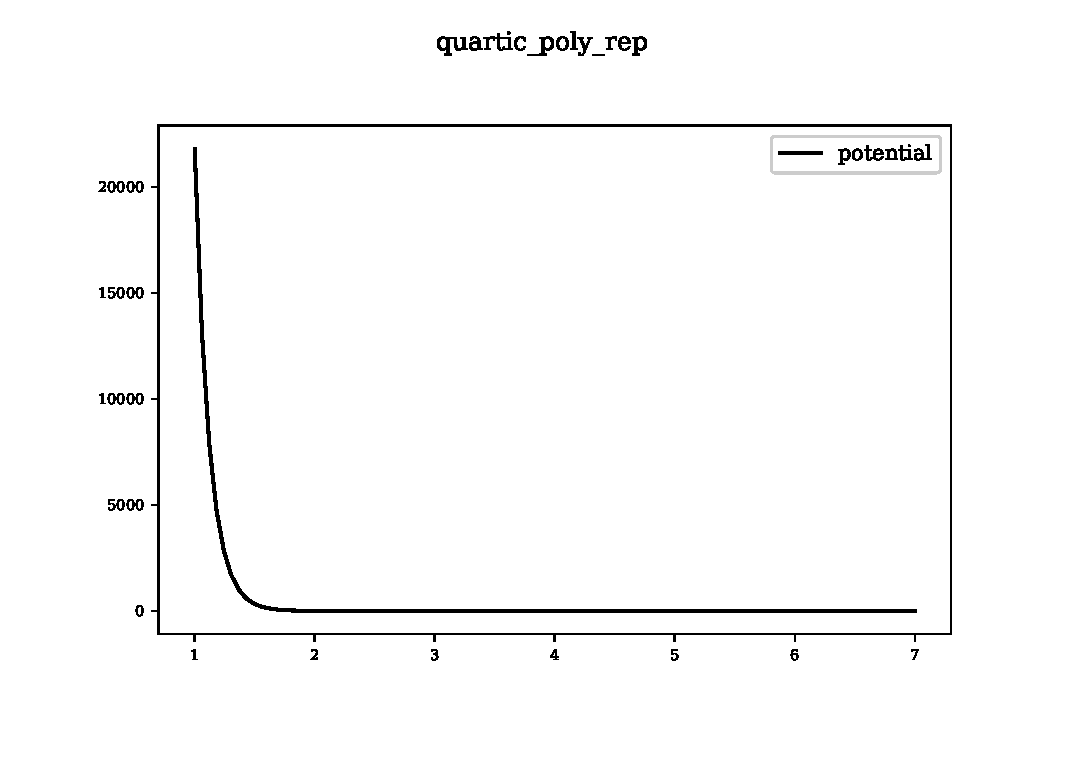
\includegraphics{img/plots/quartic_poly_rep.eps}[scale=0.6]
    \caption{Quartic Polynomial Plus Exponential Repulsion}
    \label{graph:graph1}
  \end{center}
\end{figure}

\begin{equation}
\begin{split}
H(x) = \left\{ \begin{matrix} (r - r_c)^2 (c_1 + c_1 r + c_2 r^2) + D exp(- \frac{r}{q}) & r <= r_c \\  0 & r > r_c \end{matrix} \right . 
\end{split}
\label{eq:simpleSpline}
\end{equation}

\begin{lstlisting}[style=pseudocode,caption={Quartic Polynomial with Repulsive Term}]
#A
#TYPE quartic_poly_rep
#P -4.5377 4.0659 -0.8548 9.5272e7 0.1193
#L 0.0
#U 7.0
\end{lstlisting}







\section{Density Functions}

\subsection{Quadratic Density}

\begin{figure}[h]
  \begin{center}
    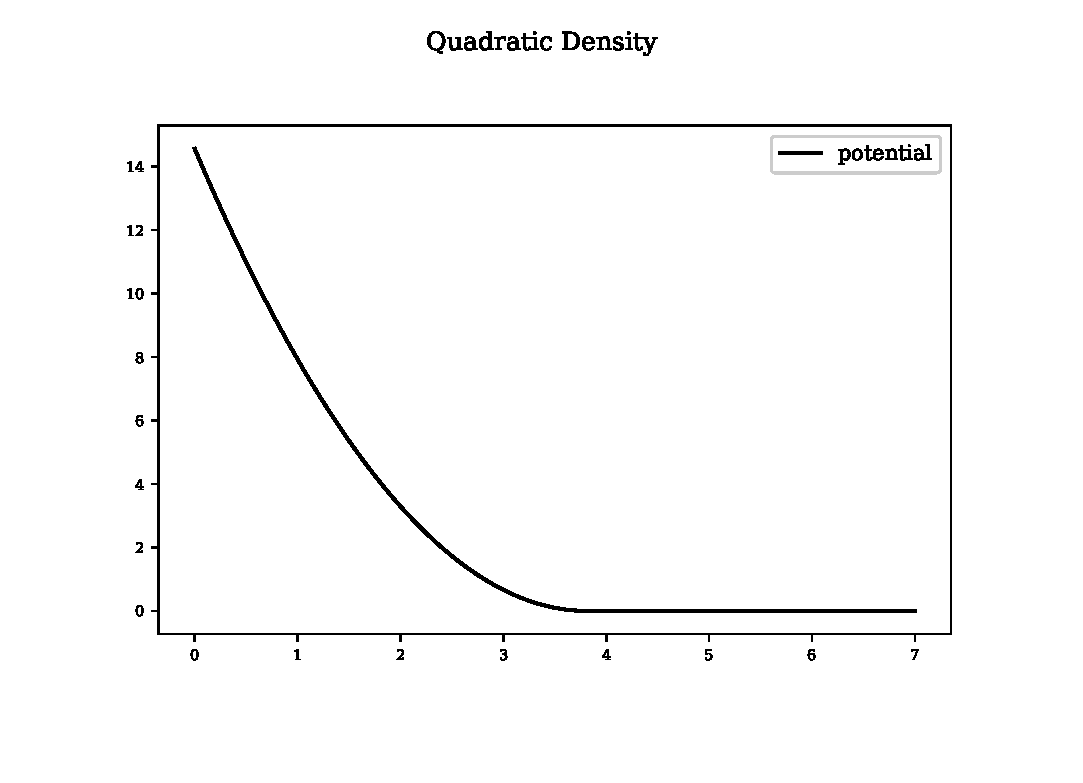
\includegraphics{img/plots/quadratic_density.eps}[scale=0.6]
    \caption{Quadratic Density}
    \label{graph:graph1}
  \end{center}
\end{figure}

\begin{equation}
\begin{split}
\rho(r) = (r - r_c)^2 
\end{split}
\label{eq:quadraticDensity}
\end{equation}

\begin{lstlisting}[style=pseudocode,caption={Quadratic Density}]
#A
#TYPE quadratic_density
#P 3.816
#L 0.0
#U 7.0
\end{lstlisting}


\subsection{Slater 4S (Squared)}

\begin{figure}[h]
  \begin{center}
    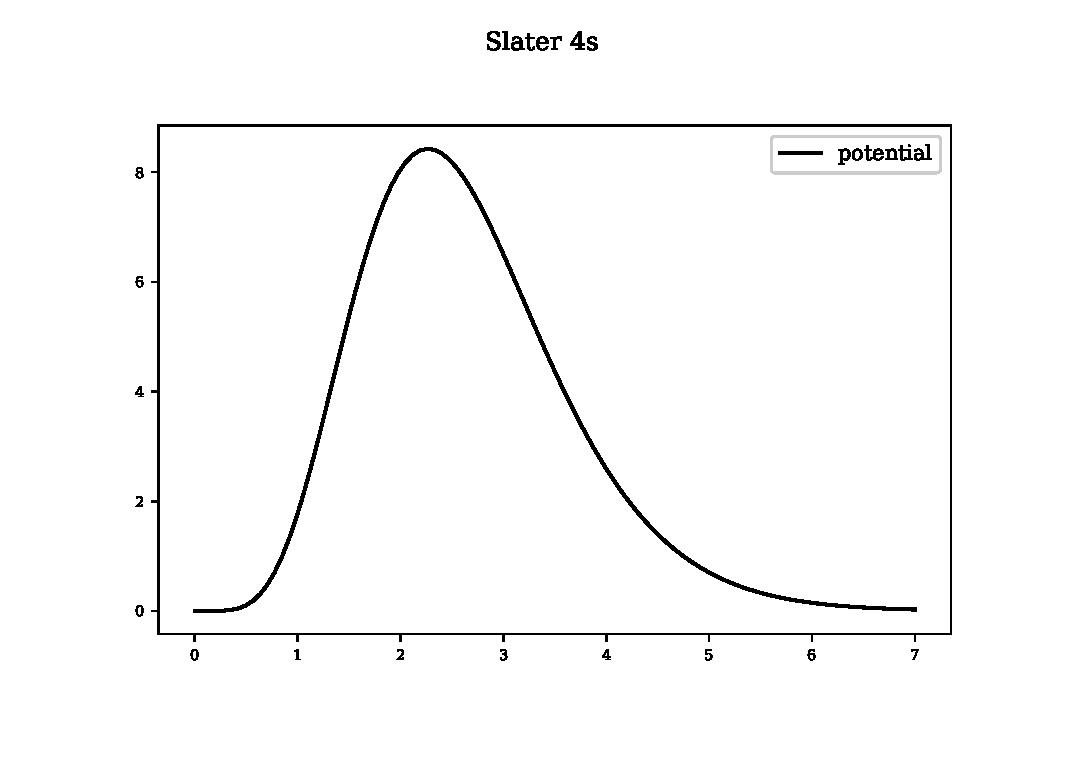
\includegraphics{img/plots/slater_4s.eps}[scale=0.6]
    \caption{Quadratic Density}
    \label{graph:graph1}
  \end{center}
\end{figure}

\begin{equation}
\begin{split}
\rho(r) = (N_s r^3 exp(-\eta r))^2 
\end{split}
\label{eq:slater4S}
\end{equation}

\begin{lstlisting}[style=pseudocode,caption={Slater 4S}]
#A
#TYPE slater_4s
#P 5.0 1.323
#L 0.0
#U 7.0
\end{lstlisting}








\section{Embedding Functions}

\subsection{Finnis-Sinclair Embedding}

\begin{figure}[h]
  \begin{center}
    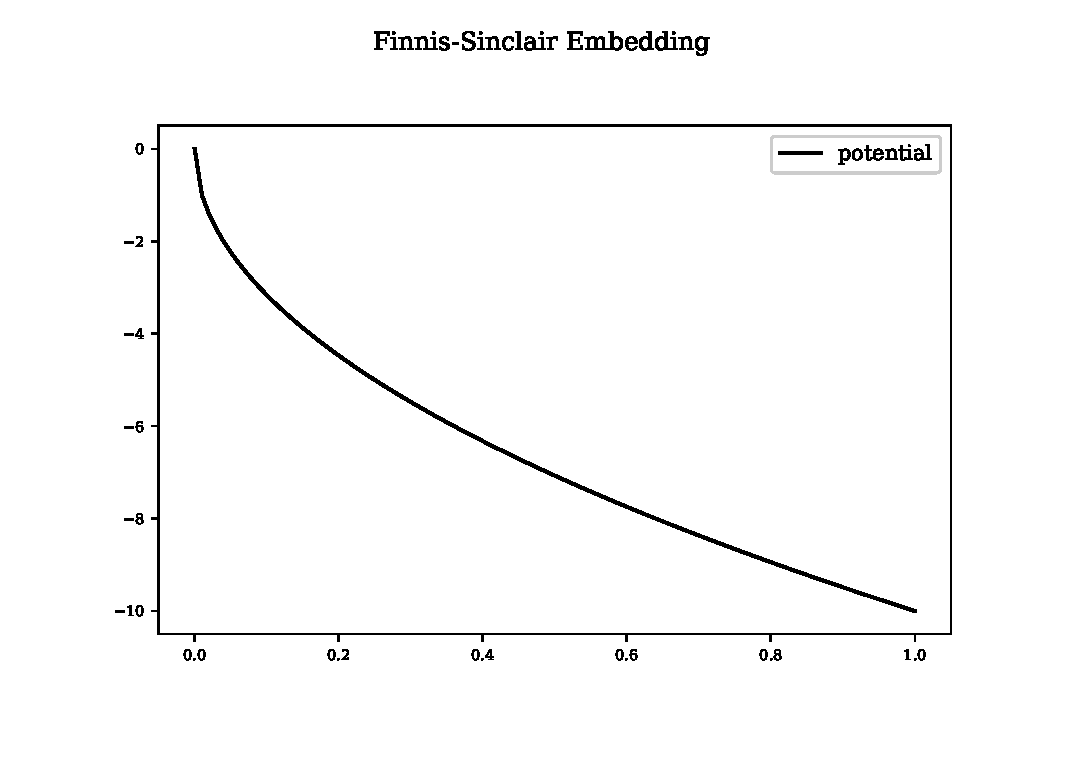
\includegraphics{img/plots/fs_embedding.eps}[scale=0.6]
    \caption{Finnis-Sinclair Embedding}
    \label{graph:graph1}
  \end{center}
\end{figure}

\begin{equation}
\begin{split}
F[\rho] = -A \sqrt(\rho)
\end{split}
\label{eq:fsEmbedding}
\end{equation}

\begin{lstlisting}[style=pseudocode,caption={Finnis-Sinclair Embedding}]
#A
#TYPE fs_embedding
#P 10.0
#L 0.0
#U 7.0
\end{lstlisting}


\subsection{Mendelev Embedding}

\begin{figure}[h]
  \begin{center}
    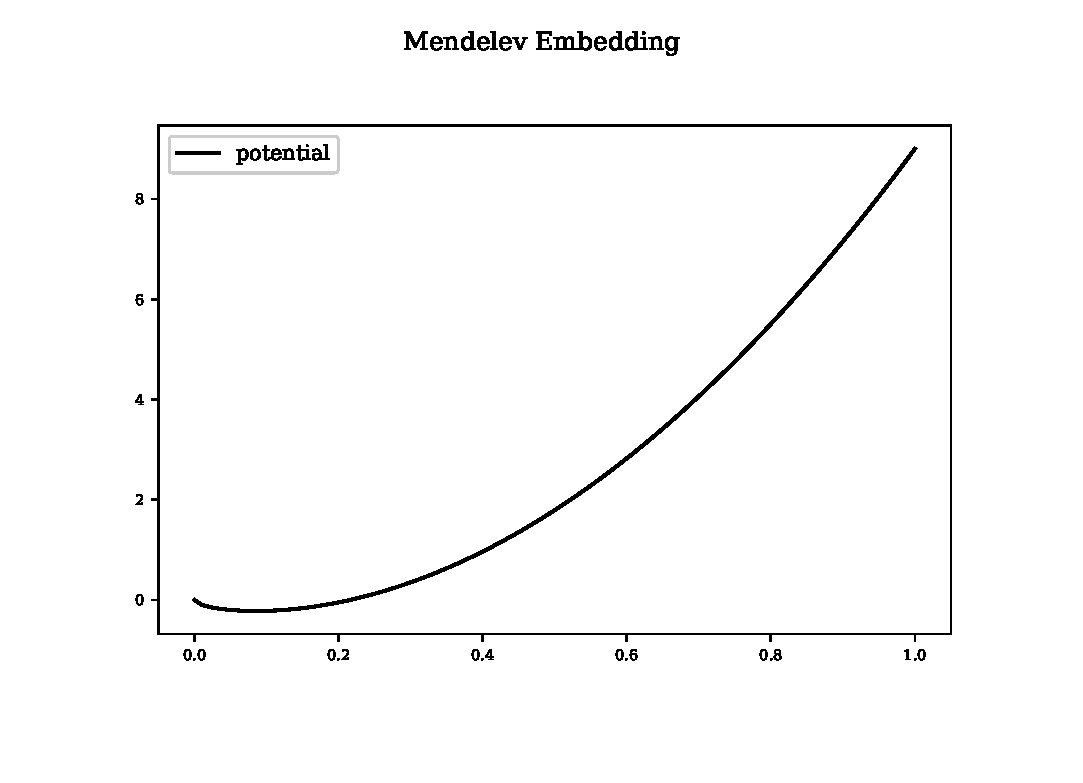
\includegraphics{img/plots/mendelev_embedding.eps}[scale=0.6]
    \caption{Mendelev Embedding}
    \label{graph:graph1}
  \end{center}
\end{figure}

\begin{equation}
\begin{split}
F[\rho] = - \sqrt(\rho) + A \rho^2
\end{split}
\label{eq:mendelevEmbedding}
\end{equation}

\begin{lstlisting}[style=pseudocode,caption={Mendelev Embedding}]
#A
#TYPE mendelev_embedding
#P 10.0
#L 0.0
#U 7.0
\end{lstlisting}


\subsection{Triple Embedding}

\begin{figure}[h]
  \begin{center}
    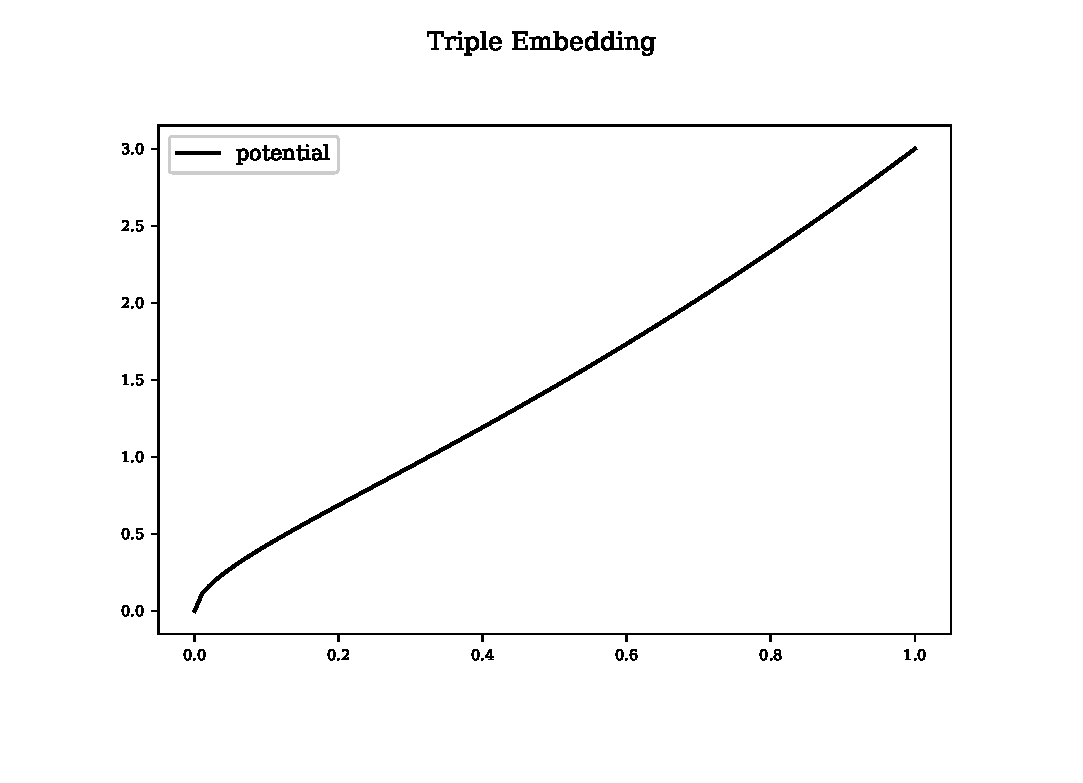
\includegraphics{img/plots/triple_embedding.eps}[scale=0.6]
    \caption{Triple Embedding}
    \label{graph:graph1}
  \end{center}
\end{figure}

\begin{equation}
\begin{split}
F[\rho] = A \sqrt(\rho) + B \rho + C \rho^2
\end{split}
\label{eq:tripleEmbedding}
\end{equation}

\begin{lstlisting}[style=pseudocode,caption={Triple Embedding}]
#A
#TYPE triple_embedding
#P 1.0 1.0 1.0
#L 0.0
#U 7.0
\end{lstlisting}



\subsection{Ackland Embedding}

\begin{figure}[h]
  \begin{center}
    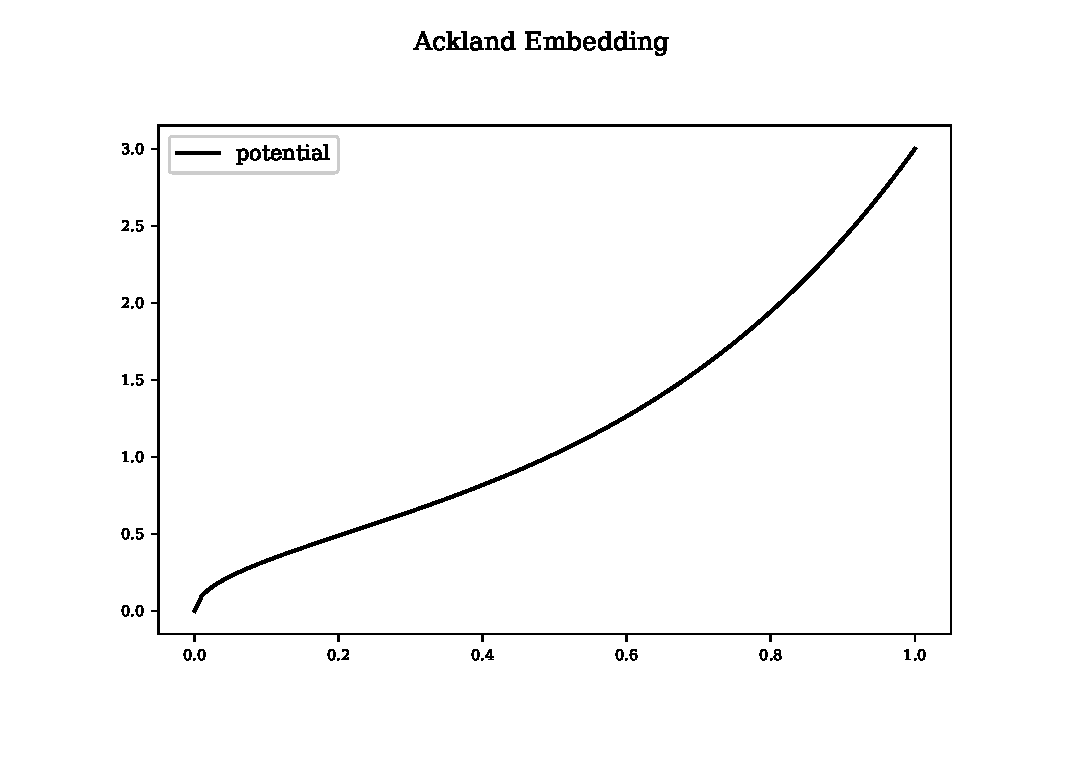
\includegraphics{img/plots/ackland_embedding.eps}[scale=0.6]
    \caption{Ackland Embedding}
    \label{graph:graph1}
  \end{center}
\end{figure}

\begin{equation}
\begin{split}
F[\rho] = A \sqrt(\rho) + B \rho^2 + C \rho^4
\end{split}
\label{eq:acklandEmbedding}
\end{equation}

\begin{lstlisting}[style=pseudocode,caption={Ackland Embedding}]
#A
#TYPE ackland_embedding
#P 1.0 1.0 1.0
#L 0.0
#U 7.0
\end{lstlisting}











\section{Generic Functions}


\subsection{Cubic Splines}

\begin{figure}[h]
  \begin{center}
    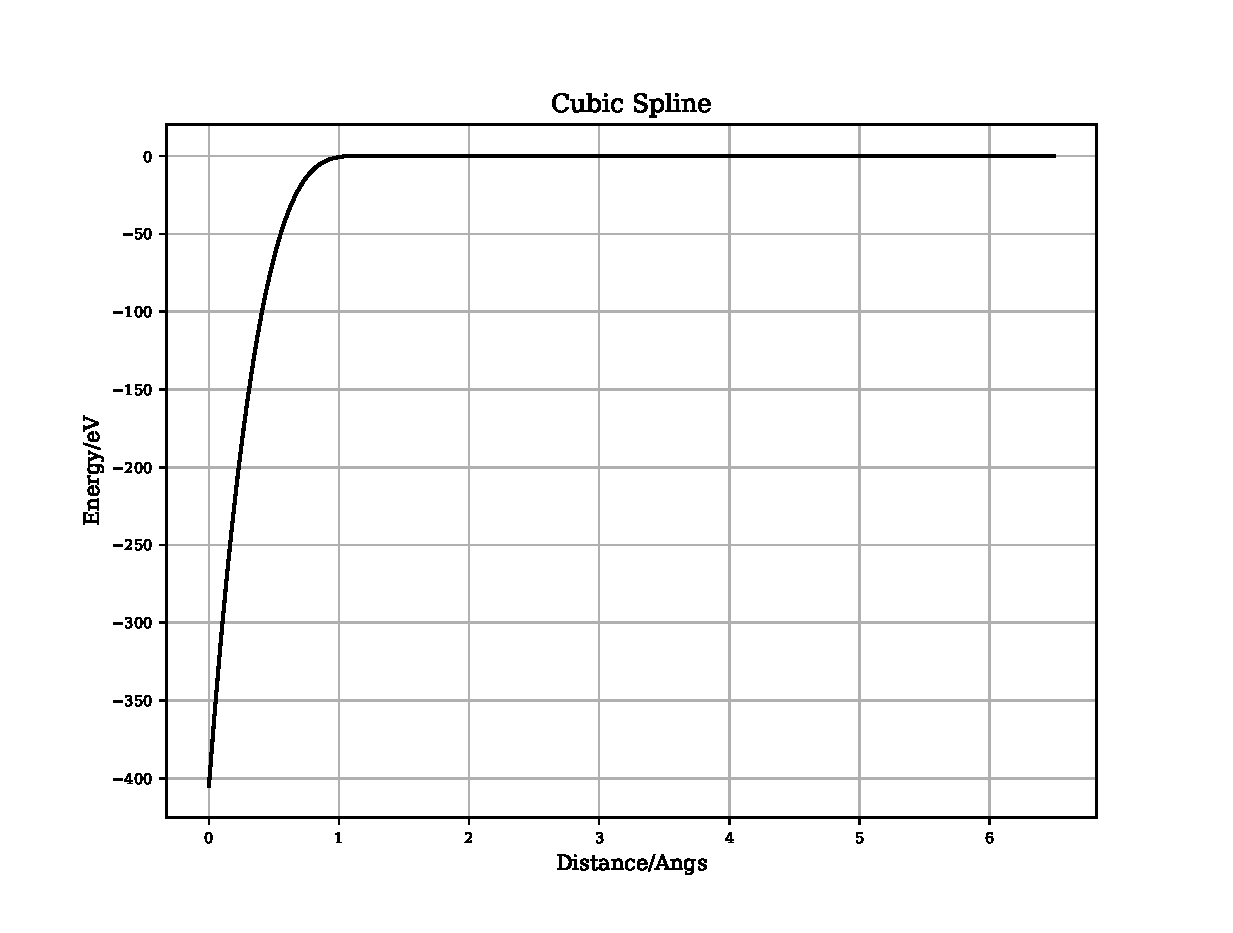
\includegraphics{img/plots/cubic_spline.eps}[scale=0.6]
    \caption{Ackland Embedding}
    \label{graph:graph1}
  \end{center}
\end{figure}

\begin{equation}
\begin{split}
V(r) = \sum_i^N a_i (r - r_i)^3 H(r_i - r) \\
\text{where } \\
H(x) = \left\{ \begin{matrix} 0 & x<0 \\  1 & x >= 0 \end{matrix} \right . 
\end{split}
\label{eq:cubicSpline}
\end{equation}

This function requires two sets of parameters.  P is a list of N coefficients and PF is a list of N cutoffs.  The cubic polynomials are summed and individually scaled by the coefficients, and by virtue of its form and the heaviside step function, they cut off at the desired radius. 

\begin{lstlisting}[style=pseudocode,caption={Cubic Splines}]
#A
#TYPE cubic_spline
#P -165.0 -78.5 -78.15 1.868
#PF 0.976 1.15 1.216 1.650
#L 0.0
#U 7.0
\end{lstlisting}





\subsection{Quintic Splines}

\begin{figure}[h]
  \begin{center}
    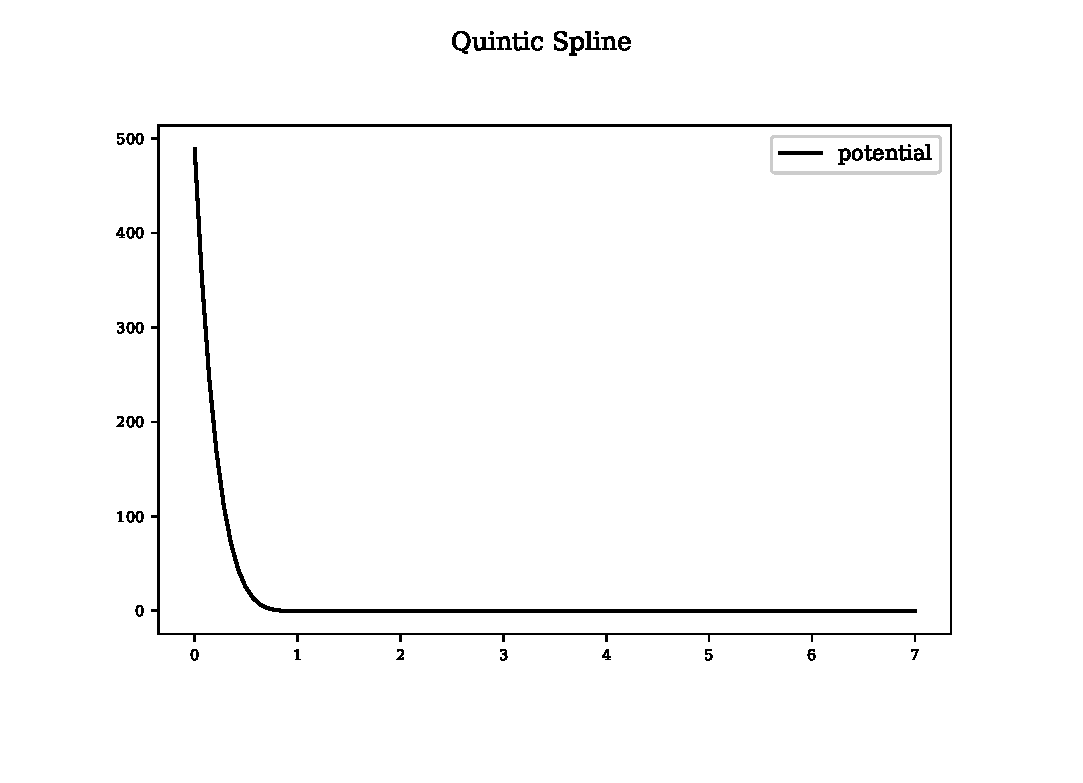
\includegraphics{img/plots/quintic_spline.eps}[scale=0.6]
    \caption{Ackland Embedding}
    \label{graph:graph1}
  \end{center}
\end{figure}

\begin{equation}
\begin{split}
V(r) = \sum_i^N a_i (r - r_i)^5 H(r_i - r) \\
\text{where } \\
H(x) = \left\{ \begin{matrix} 0 & x<0 \\  1 & x >= 0 \end{matrix} \right . 
\end{split}
\label{eq:quinticSpline}
\end{equation}

\begin{lstlisting}[style=pseudocode,caption={Quintic Splines}]
#A
#TYPE quintic_spline
#P -165.0 -78.5 -78.15 1.868
#PF 0.976 1.15 1.216 1.650
#L 0.0
#U 7.0
\end{lstlisting}





















\end{appendices}






%%######################################################################
%% Bibliography
%%######################################################################


\printbibliography









\end{document}
